\documentclass[margin=2mm]{standalone}
\usepackage{tikz}
\usepackage{circuitikz}
\usetikzlibrary{calc,positioning,shapes.geometric,backgrounds,fit,shadows.blur,arrows,arrows.meta,decorations.markings}
\tikzset{
  hole/.style = {fill = #1, circle, minimum width = 2.5mm, inner sep = 0mm},
  wire/.style = {draw = #1, line width = .5mm},
  line/.style={-,line width = 3},
  label/.style = {black!50!white, font=\sffamily, anchor = center},
  text/.style = {white, font=\sffamily, anchor = right},
}
\begin{document}
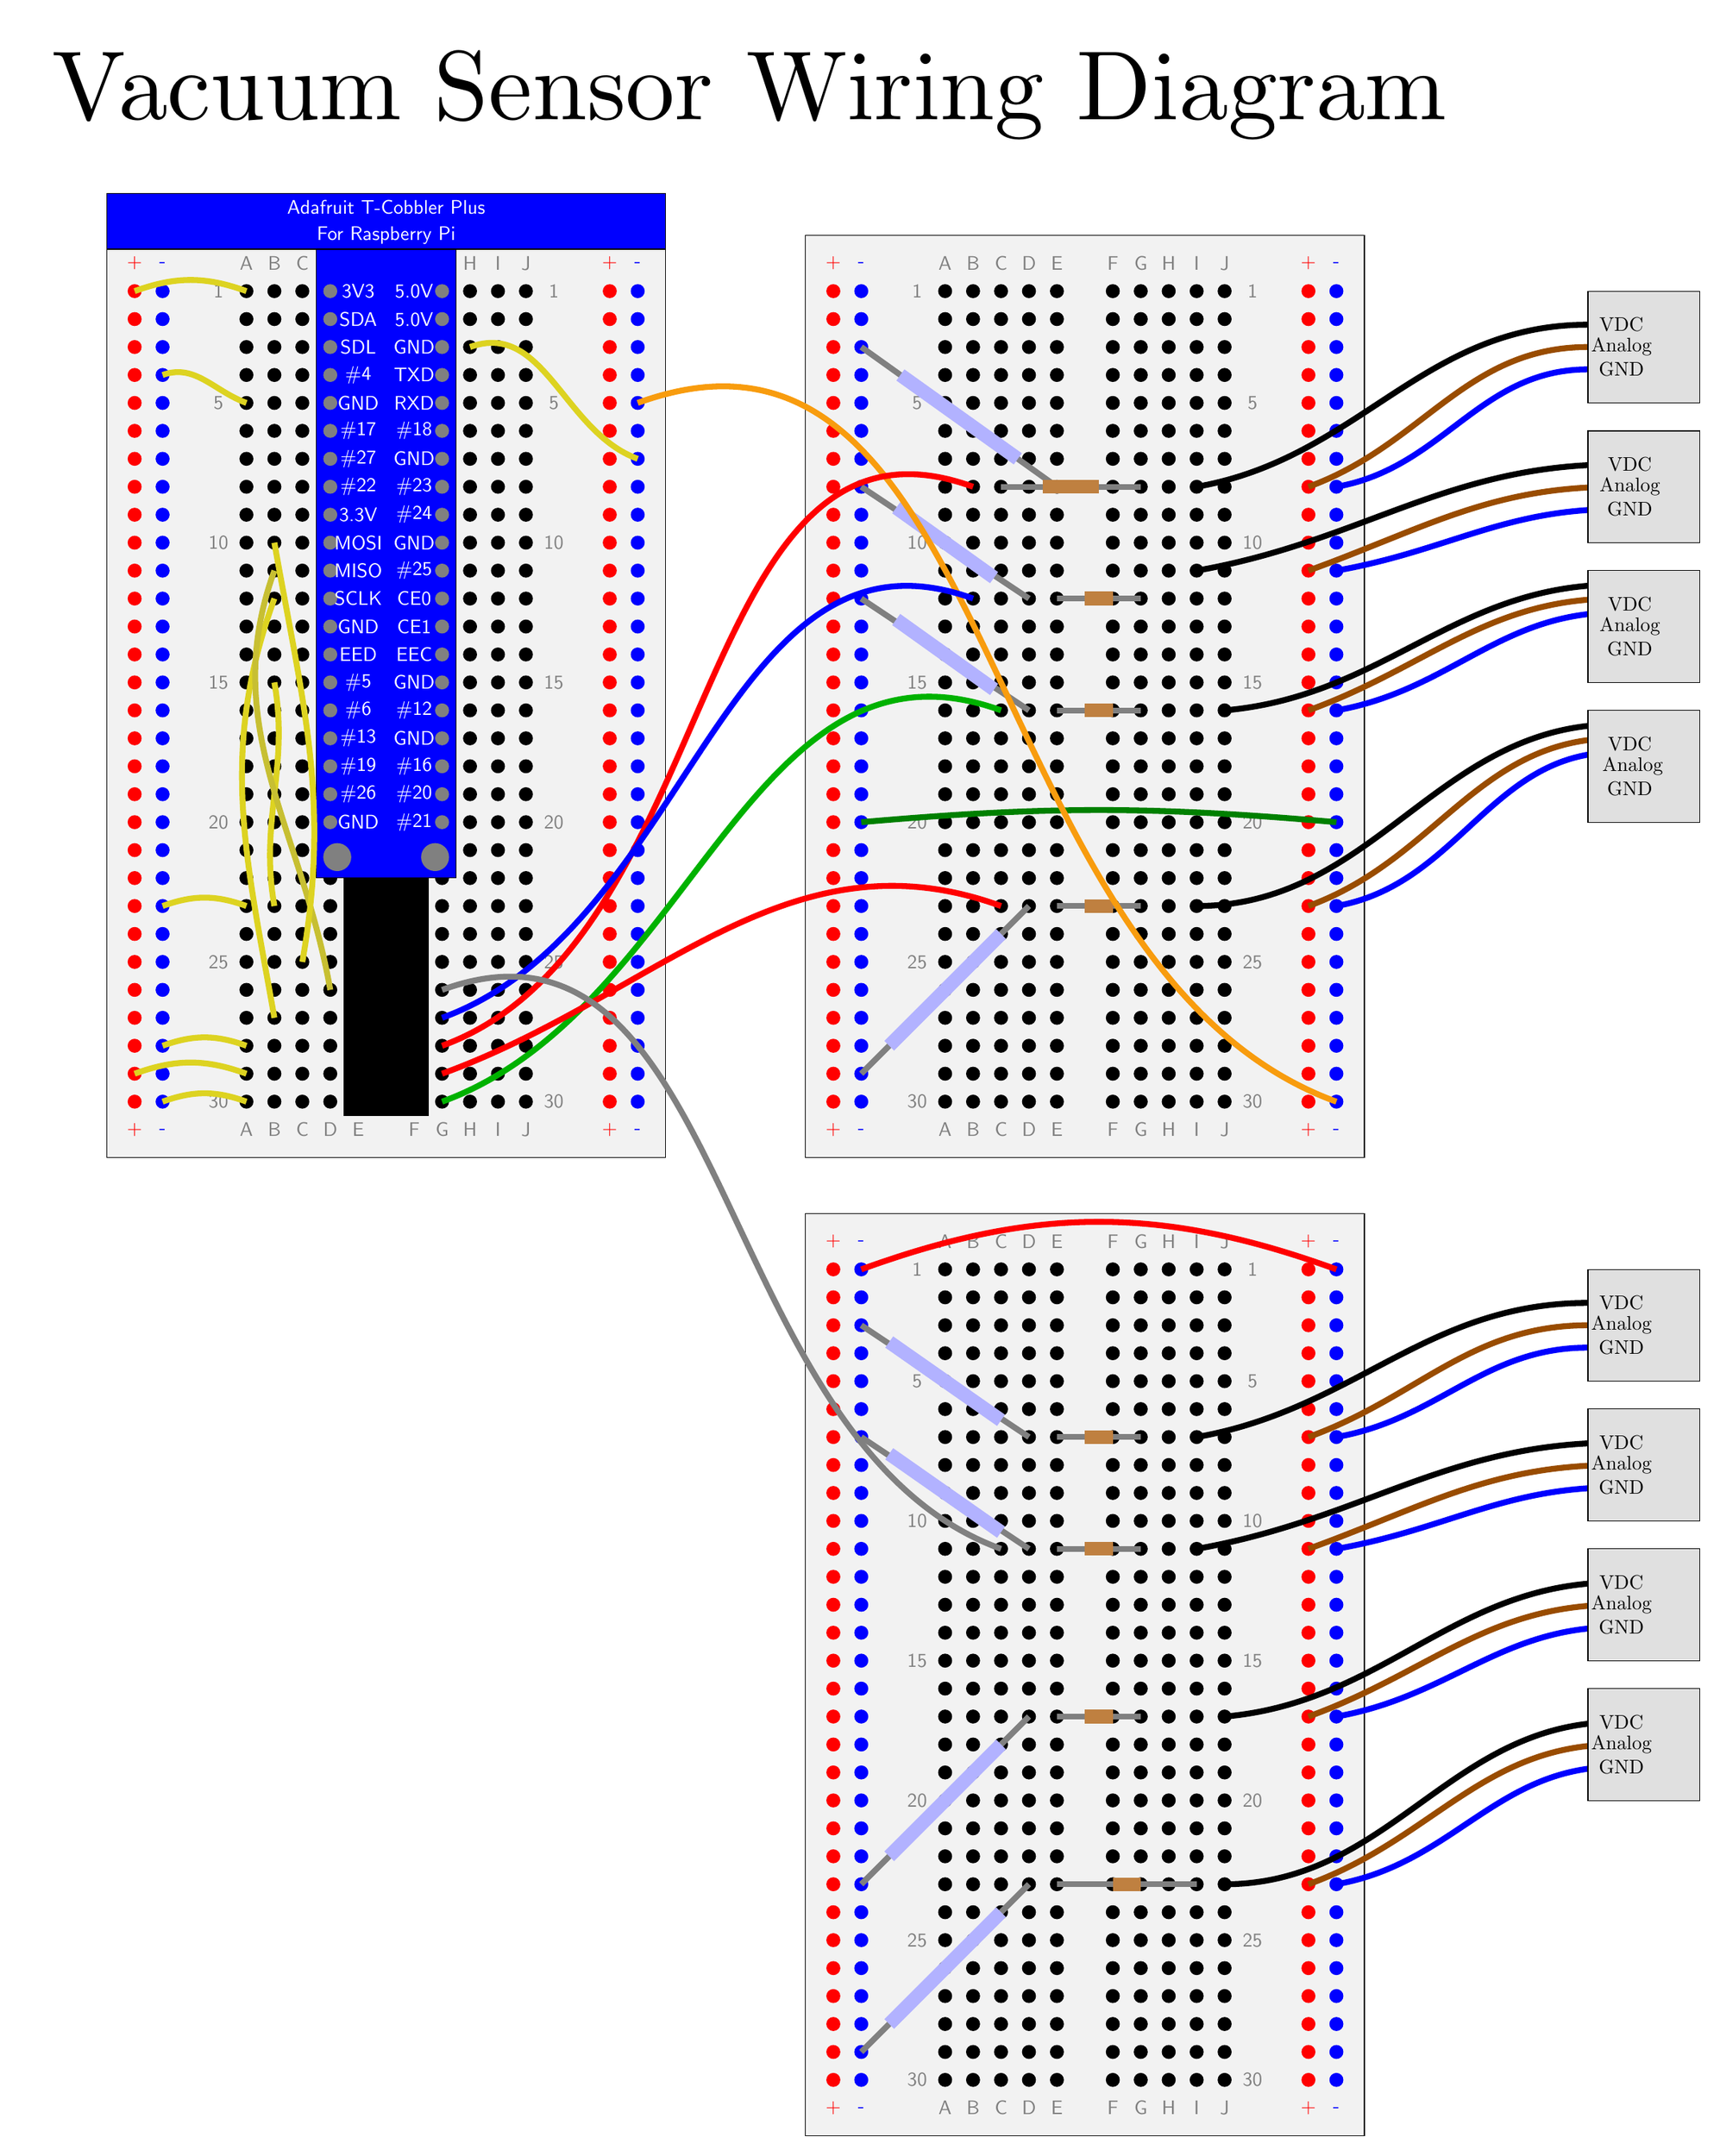
\begin{tikzpicture}[x= 5mm,y=5mm]
  % Vacuum Sensor Wiring
  \node[scale=5] at (-6,37) {Vacuum Sensor Wiring Diagram};
  % breadboard1
  \draw[fill=black!05!white] (-4,-1) rectangle (16,32);
  % \draw[wire=red]  (-3,1) -- (-3,30);
  % \draw[wire=blue] (-2,1) -- (-2,30);
  % \draw[wire=red]  (14,1) -- (14,30);
  % \draw[wire=blue] (15,1) -- (15,30);
  \foreach \yi in {1,...,30}{
    \node[hole=red]  at (-3,\yi){};
    \node[hole=blue] at (-2,\yi){};
    \node[hole=red]  at (14,\yi){};
    \node[hole=blue] at (15,\yi){};
    \foreach \xs in {0,6}{
      % \draw[wire=black] (\xs+1,\yi) -- (\xs+5,\yi);
      \foreach \xi in {1,2,3,4,5}{
        \node[hole=black] at (\xi+\xs,\yi){};
      }
    }
  }
  \foreach \m/\xi in {A/1,B/2,C/3,D/4,E/5,F/7,G/8,H/9,I/10,J/11}{
    \node[label=90] at (\xi,0) {\m};
    \node[label=90] at (\xi,31) {\m};
  }
  \foreach \m/\yi in {30/1,25/6,20/11,15/16,10/21,5/26,1/30}{
    \node[label=90] at (0,\yi) {\m};
    \node[label=90] at (12,\yi) {\m};
  }
  \foreach \m/\xi in {+/-3,+/14}{
    \node[red] at (\xi,0) {\m};
    \node[red] at (\xi,31) {\m};
  }
  \foreach \m/\xi in {-/-2,-/15}{
    \node[blue] at (\xi,0) {\m};
    \node[blue] at (\xi,31) {\m};
  }
  % resistors
  \draw[line,white!50!black] (-2,28) to (5,23);
  \draw[line,white!70!blue,line width=7] (-0.6,27) to (3.6,24);
  \draw[line,white!50!black] (3,23) to (8,23);
  \draw[line,brown,line width=7] (4.5,23) to (6.5,23);
  \draw[line,white!50!black] (-2,23) to (4,19);%RESISTOR2
  \draw[line,white!70!blue,line width=7] (-0.75,22.25) to (2.75,19.75);%RES2
  \draw[line,white!50!black] (5,19) to (8,19);%RES2
  \draw[line,brown,line width=7] (6,19) to (7,19);%RES2
  \draw[line,white!50!black] (-2,19) to (4,15);%RESISTOR3
  \draw[line,white!70!blue,line width=7] (-0.75,18.25) to (2.75,15.75);%RESISTOR3
  \draw[line,white!50!black] (5,15) to (8,15);%RESISTOR3
  \draw[line,brown,line width=7] (6,15) to (7,15);%RESISTOR3
  \draw[line,white!50!black] (-2,2) to (4,8);
  \draw[line,white!70!blue,line width=7] (-1,3) to (3,7);
  \draw[line,white!50!black] (5,8) to (8,8);
  \draw[line,brown,line width=7] (6,8) to (7,8);

  % vac sensor1
  \draw[line,blue] (15,23) to [out=10,in=180] (24,27.2);
  \draw[line,black!40!orange] (14,23) to [out=20,in=180] (24,28);
  \draw[line,black] (10,23) to [out=10,in=180] (24,28.8);
  \draw[fill=black!12!white] (24,26) rectangle (28,30); %BOX
  \foreach \m/\yi in {GND/27.2,Analog/28,VDC/28.8}{
    \node[align=right] at (25.2,\yi) {\m};
    }
  % vac sensor2
  \draw[line,blue] (15,20) to [out=10,in=180] (25,22.2);
  \draw[line,black!40!orange] (14,20) to [out=20,in=180] (25,23);
  \draw[line,black] (10,20) to [out=10,in=180] (25,23.8);
  \draw[fill=black!12!white] (24,21) rectangle (28,25); %BOX
  \node[scale=1] at (25.5,23.8) {VDC};
  \node[scale=1] at (25.5,23) {Analog};
  \node[scale=1] at (25.5,22.2) {GND};
    % vac sensor3
  \draw[line,blue] (15,15) to [out=10,in=180] (25,18.5);
  \draw[line,black!40!orange] (14,15) to [out=20,in=180] (25,19);
  \draw[line,black] (11,15) to [out=5,in=180] (25,19.5);
  \draw[fill=black!12!white] (24,16) rectangle (28,20); %BOX
  \node[scale=1] at (25.5,18.8) {VDC};
  \node[scale=1] at (25.5,18) {Analog};
  \node[scale=1] at (25.5,17.2) {GND};
  % vac sensor4
  \draw[line,blue] (15,8) to [out=10,in=180] (25,13.5);
  \draw[line,black!40!orange] (14,8) to [out=20,in=180] (25,14);
  \draw[line,black] (10,8) to [out=0,in=180] (25,14.5);
  \draw[fill=black!12!white] (24,11) rectangle (28,15); %BOX
  \node[scale=1] at (25.5,13.8) {VDC};
  \node[scale=1] at (25.6,13) {Analog};
  \node[scale=1] at (25.5,12.2) {GND};
  % wires
  \draw[line,black!50!green] (15,11) to [out=175,in=5] (-2,11);

  % breadboard 2
  \tikzset{shift={(0,-35)}}
  \draw[fill=black!05!white] (-4,-1) rectangle (16,32);
  % \draw[wire=red]  (-3,1) -- (-3,30);
  % \draw[wire=blue] (-2,1) -- (-2,30);
  % \draw[wire=red]  (14,1) -- (14,30);
  % \draw[wire=blue] (15,1) -- (15,30);
  \foreach \yi in {1,...,30}{
    \node[hole=red]  at (-3,\yi){};
    \node[hole=blue] at (-2,\yi){};
    \node[hole=red]  at (14,\yi){};
    \node[hole=blue] at (15,\yi){};
    \foreach \xs in {0,6}{
      % \draw[wire=black] (\xs+1,\yi) -- (\xs+5,\yi);
      \foreach \xi in {1,2,3,4,5}{
        \node[hole=black] at (\xi+\xs,\yi){};
      }
    }
  }
  \foreach \m/\xi in {A/1,B/2,C/3,D/4,E/5,F/7,G/8,H/9,I/10,J/11}{
    \node[label=90] at (\xi,0) {\m};
    \node[label=90] at (\xi,31) {\m};
  }
  \foreach \m/\yi in {30/1,25/6,20/11,15/16,10/21,5/26,1/30}{
    \node[label=90] at (0,\yi) {\m};
    \node[label=90] at (12,\yi) {\m};
  }
  \foreach \m/\xi in {+/-3,+/14}{
    \node[red] at (\xi,0) {\m};
    \node[red] at (\xi,31) {\m};
  }
  \foreach \m/\xi in {-/-2,-/15}{
    \node[blue] at (\xi,0) {\m};
    \node[blue] at (\xi,31) {\m};
  }
  \draw[line,white!50!black] (-2,28) to (4,24);%blue resistor 1
  \draw[line,white!70!blue,line width=7] (-1,27.4) to (3,24.6);%blue 1
  \draw[line,white!50!black] (5,24) to (8,24);%brown1
  \draw[line,brown,line width=7] (6,24) to (7,24);%brown1
  \draw[line,white!50!black] (-2,24) to (4,20);%blue 2
  \draw[line,white!70!blue,line width=7] (-1,23.4) to (3,20.6);%blue2
  \draw[line,white!50!black] (5,20) to (8,20);%brown2
  \draw[line,brown,line width=7] (6,20) to (7,20);%brown2
  \draw[line,white!50!black] (-2,8) to (4,14);%Blue3
  \draw[line,white!70!blue,line width=7] (-1,9) to (3,13);%blue3
  \draw[line,white!50!black] (5,14) to (8,14);%brown3
  \draw[line,brown,line width=7] (6,14) to (7,14);%brown3
  \draw[line,white!50!black] (-2,2) to (4,8);%blue4
  \draw[line,white!70!blue,line width=7] (-1,3) to (3,7);%blue4
  \draw[line,white!50!black] (5,8) to (10,8);%brown4
  \draw[line,brown,line width=7] (7,8) to (8,8);%brown4
  \draw[line,red] (-2,30) to [out=20,in=160] (15,30);%brown1


% vac sensor1 bb2
  \draw[line,blue] (15,24) to [out=10,in=180] (24,27.2);
  \draw[line,black!40!orange] (14,24) to [out=20,in=180] (24,28);
  \draw[line,black] (10,24) to [out=10,in=180] (24,28.8);
  \draw[fill=black!12!white] (24,26) rectangle (28,30); %BOX
  \foreach \m/\yi in {GND/27.2,Analog/28,VDC/28.8}{
    \node[align=right] at (25.2,\yi) {\m};
    }
  % vac sensor2  bb2
  \draw[line,blue] (15,20) to [out=10,in=180] (25,22.2);
  \draw[line,black!40!orange] (14,20) to [out=20,in=180] (25,23);
  \draw[line,black] (10,20) to [out=10,in=180] (25,23.8);
  \draw[fill=black!12!white] (24,21) rectangle (28,25); %BOX
  \node[scale=1] at (25.2,23.8) {VDC};
  \node[scale=1] at (25.2,23) {Analog};
  \node[scale=1] at (25.2,22.2) {GND};
    % vac sensor3  bb2
  \draw[line,blue] (15,14) to [out=10,in=180] (25,17.2);
  \draw[line,black!40!orange] (14,14) to [out=20,in=180] (25,18);
  \draw[line,black] (11,14) to [out=5,in=180] (25,18.8);
  \draw[fill=black!12!white] (24,16) rectangle (28,20); %BOX
  \node[scale=1] at (25.2,18.8) {VDC};
  \node[scale=1] at (25.2,18) {Analog};
  \node[scale=1] at (25.2,17.2) {GND};
  % vac sensor4  bb2
  \draw[line,blue] (15,8) to [out=10,in=180] (25,12.2);
  \draw[line,black!40!orange] (14,8) to [out=20,in=180] (25,13);
  \draw[line,black] (11,8) to [out=0,in=180] (25,13.8);
  \draw[fill=black!12!white] (24,11) rectangle (28,15); %BOX
  \node[scale=1] at (25.2,13.8) {VDC};
  \node[scale=1] at (25.2,13) {Analog};
  \node[scale=1] at (25.2,12.2) {GND};


  % breadboard 3
  \tikzset{shift={(-25,35)}}
  \draw[fill=black!05!white] (-4,-1) rectangle (16,32);
  % \draw[wire=red]  (-3,1) -- (-3,30);
  % \draw[wire=blue] (-2,1) -- (-2,30);
  % \draw[wire=red]  (14,1) -- (14,30);
  % \draw[wire=blue] (15,1) -- (15,30);
  \foreach \yi in {1,...,30}{
    \node[hole=red]  at (-3,\yi){};
    \node[hole=blue] at (-2,\yi){};
    \node[hole=red]  at (14,\yi){};
    \node[hole=blue] at (15,\yi){};
    \foreach \xs in {0,6}{
      % \draw[wire=black] (\xs+1,\yi) -- (\xs+5,\yi);
      \foreach \xi in {1,2,3,4,5}{
        \node[hole=black] at (\xi+\xs,\yi){};
      }
    }
  }
  \foreach \m/\xi in {A/1,B/2,C/3,D/4,E/5,F/7,G/8,H/9,I/10,J/11}{
    \node[label=90] at (\xi,0) {\m};
    \node[label=90] at (\xi,31) {\m};
  }
  \foreach \m/\yi in {30/1,25/6,20/11,15/16,10/21,5/26,1/30}{
    \node[label=90] at (0,\yi) {\m};
    \node[label=90] at (12,\yi) {\m};
  }
  \foreach \m/\xi in {+/-3,+/14}{
    \node[red] at (\xi,0) {\m};
    \node[red] at (\xi,31) {\m};
  }
  \foreach \m/\xi in {-/-2,-/15}{
    \node[blue] at (\xi,0) {\m};
    \node[blue] at (\xi,31) {\m};
  }
% T Cobbler
  \draw[fill=blue] (-4,31.5) rectangle (16,33.5);
  \draw[fill=blue] (3.5,31.5) rectangle (8.5,9);
  \draw[fill=black] (4.5,9) rectangle (7.5,0.5);
  \foreach \yi in {11,...,30}{
    \node[hole=gray] at (4,\yi){};
    \node[hole=gray] at (8,\yi){};
  }
  \foreach \m/\yi in {3V3/30,SDA/29,SDL/28,\#4/27,GND/26,\#17/25,\#27/24,\#22/23,3.3V/22,MOSI/21,MISO/20,SCLK/19,GND/18,EED/17,\#5/16,\#6/15,\#13/14,\#19/13,\#26/12,GND/11}{ 
    \node[white, font=\sffamily, align=right] at (5,\yi) {\m};
  }
  \foreach \m/\yi in {5.0V/30,5.0V/29,GND/28,TXD/27,RXD/26,\#18/25,GND/24,\#23/23,\#24/22,GND/21,\#25/20,CE0/19,CE1/18,EEC/17,GND/16,\#12/15,GND/14,\#16/13,\#20/12,\#21/11}{ 
    \node[white, font=\sffamily, align= left] at (7,\yi) {\m};
  }
  \node[white, font=\sffamily] at (6,33) {Adafruit T-Cobbler Plus};
  \node[white, font=\sffamily] at (6,32) {For Raspberry Pi};
  \foreach \x in {4.25,7.75}{
    \node[fill = gray, circle, minimum width = 5mm, inner sep = 1mm] at (\x,9.75){};
  }
  \draw[line,yellow!85!black] (-3,30) to [out=20,in=160] (1,30);  
  \draw[line,yellow!85!black] (-2,27) to [out=20,in=160] (1,26);  
  \draw[line,yellow!85!black] (9,28) to [out=20,in=160] (15,24);
  \draw[line,yellow!85!black] (-2,8) to [out=20,in=160] (1,8); 
  \draw[line,yellow!85!black] (2,16) to [out=280,in=100] (2,8); 
  \draw[line,yellow!85!black] (2,19) to [out=250,in=100] (2,4); 
  \draw[line,yellow!75!black] (2,20) to [out=250,in=100] (4,5);
  \draw[line,yellow!85!black] (2,21) to [out=280,in=80] (3,6);
  \draw[line,yellow!85!black] (-2,3) to [out=20,in=160] (1,3); 
  \draw[line,yellow!85!black] (-3,2) to [out=20,in=160] (1,2); 
  \draw[line,yellow!85!black] (-2,1) to [out=20,in=160] (1,1);


  \draw[line,yellow!60!red] (15,26) to [out=20,in=160] (40,1);%board to board gnd
  \draw[line,green!70!black] (8,1) to [out=20,in=160] (28,15);%board to board dev
  \draw[line,red] (8,2) to [out=20,in=160] (28,8);%board to board dev
  \draw[line,red] (8,3) to [out=20,in=160] (27,23);%board to board dev
  \draw[line,blue] (8,4) to [out=20,in=160] (27,19);%board to board dev
  \draw[line,white!50!black] (8,5) to [out=20,in=160] (28,-15);%board to board dev
  

  
  % % grid indicator
  % \tikzset{shift={(0,-35)}}
  % \draw[fill=black!05!white] (-4,-1) rectangle (16,32);
  % \foreach \yi in {1,...,30}{
  %   \node[hole=red]  at (-3,\yi){};
  %   \node[hole=blue] at (-2,\yi){};
  %   \node[hole=red]  at (14,\yi){};
  %   \node[hole=blue] at (15,\yi){};
  %   \foreach \xs in {0,6}{
  %     \foreach \xi in {1,2,3,4,5}{
  %       \node[hole=black] at (\xi+\xs,\yi){};
  %     }
  %   }
  % }
  % \foreach \m/\yi in {30/1,25/6,20/11,15/16,10/21,5/26,1/30}{
  %   \node[label=90] at (12,\yi) {\m};
  % }
  % \foreach \xi in {-3,-2,-1,...,14,15,}{
  %   \node[scale=1.25] at (\xi,0) {\xi};
  % }
  % \foreach \yi in {0,1,2,...,31}{
  %   \node[scale=1.25] at (0,\yi) {\yi};
  % }
\end{tikzpicture}
\end{document}
\end{tikzpicture}
\end{document}

